\section{香港認同是怎樣開始的?}

香港認同的起點,在於香港人意識到自己雖然和中國大陸相關,卻又有所不同。

在中國大陸討論香港政治,很多時候都會聽到「因為中國和香港的社會文化同源,香港理應是中國一部分」的說法。到底兩個文化要有多大的差異我們才能將其政治上的分或合視為合理,其實從來沒有客觀標準。畢竟,世上兩處文化相異卻同為一國,或兩處文化相近卻分為兩國的例子,數之不盡。美國獨立的時候,搞獨立運動的那班人和他們要脫離的英國皇室一樣都講英文,不見得有人會聲稱「既然說英文就要承認自己是英國人」;與此同時,現在的美國沒有法定語言,在紐約州考駕駛執照可以用十三種語言回答筆試,又不見得美國因此面對分裂危機。很明顯,文化和認同的關係並非必然;與其強求定義,不如讓當地人自己回答更為合適。一個地方的內在認同,來自當地人對自身的探索,香港人和香港認同也不例外。

要討論香港人的香港故事,並不是因為來自香港本土的香港故事特別準確。正如自傳通常都都帶有十分明顯的主觀判斷,香港人自己寫的香港故事難免都會隱含大量偏見。被傳訟的香港故事難免都會被主流觀點所壟斷,少數人的聲音例如少數族裔的故事通常都被忽視。不過在認識到這些限制的前提下,討論香港人身分認同仍然是理解香港眾多社會現象的重要線索。

有關身分認同的研究,往往會由人口政策、文化產品和政治背景說起。

人口的流動和人口結構的改變,對身分認同起決定作用。不同年齡的人因為經歷過的社會事件不一樣,會產生不同的身分認同。香港作為一個移民社會,要訴說香港人的身分認同,也不得不先從人口說起。由二次大戰完結到八十年代初,中英就香港前途展開談判期間,香港的人口結構起了翻天覆地的變化,而這變化可謂直接決定了後來香港社會的精神面貌。

當香港於一九四一年被日軍佔領的時候,人口有一百多萬。到了一九四五年二戰結束,因為戰時不少人返鄉避難,香港人口只剩約六十萬人。然而到了一九四九年,人口總數卻暴增至二百二十萬。很明顯,這些新增人口不可能全都是在戰爭期間離港避難的香港居民,或戰後在港出生的嬰兒。他們更多是首次從中國大陸來到香港的移民,也就是說當時每四個人就有三個是移民。

\begin{figure}[htbp]
    \centering
    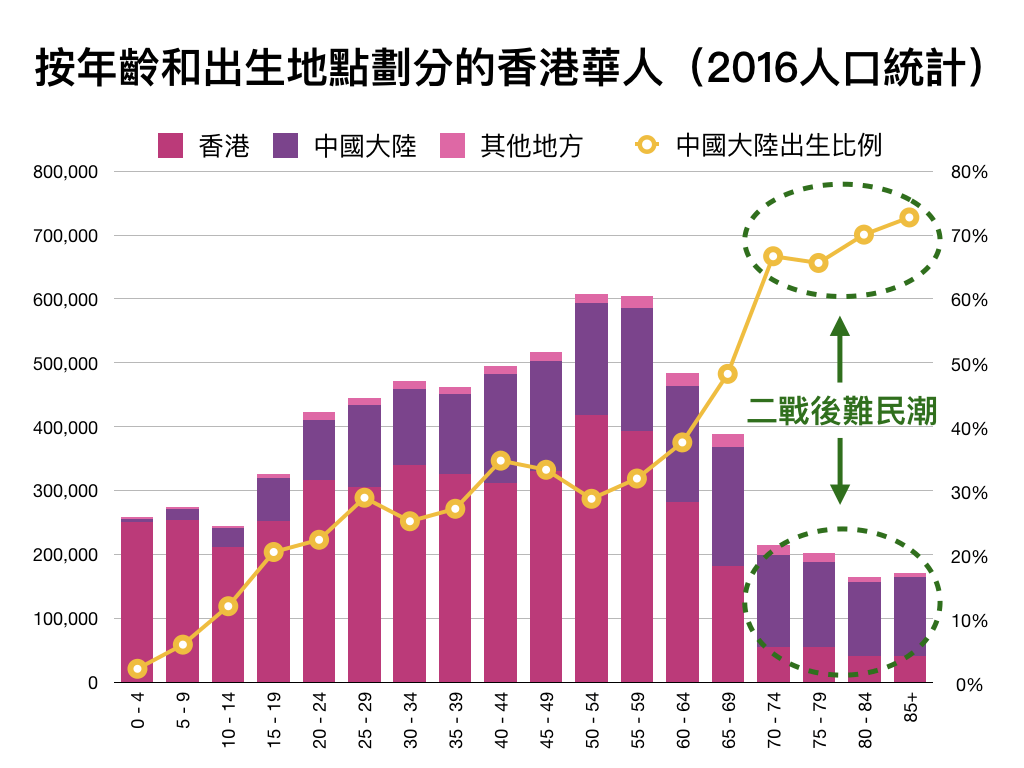
\includegraphics[width=0.7\textwidth]{c04/h-klesson1-003.png}
    \caption{二戰後難民潮對香港人口結構的影響} 
\end{figure}

讓我們把目光放遠一點。正正在這五年間,中國大陸的內戰形勢逆轉,共產黨戰勝了國民黨。大批國民黨人、資本家、文人以至一般老百姓為了逃避共產黨而前來香港,組成了戰後香港人口的主要部分。回顧這段歷史,我們可以說:所謂香港人,就是一群因為害怕共產黨而逃出中國大陸的人,及其後代。從這句話出發,很多香港人的特質和對中國大陸的態度,以至香港社會中的各種現象,都變得有跡可尋。

這些百萬計的南來避難者當中,有來自上海的資本家帶著資本和企業精神來港,大大推動了戰後香港的工商業發展。香港特區第一任行政長官董建華,本身就是上海出生,剛好正是在一九四九年,也就是他十二歲的時候隨父親董浩雲來港。董浩雲本身在上海的時候創立了中國航運公司,來港後又創立了東方海外有限公司,繼續國際航運事業。除了航運業,早期香港最先發展起來的有紡織業,著名企業有江蘇唐炳源來港設立的南海紡織,後來又有上海查濟民成立的中國染廠和陳廷驊的南豐紡織。當時的紡織業可謂都是上海華商的天下。

此外,避難者當中還有不少文人,如毛澤東在《丢掉幻想,準備鬥爭》一文中點名批判的中國史學大師錢穆。他和當代哲學家唐君毅及其他南來文人在香港創辦了新亞書院,而新亞書院後來成為了香港中文大學的創校成員之一。香港中文大學的另外兩所創校成員,即聯合書院和崇基學院,同樣有中國大陸的密切淵源,沿自於從中國大陸高等院校南遷至港的師生,如上海聖約翰大學和金陵女子大學等。

再說下去,還有數之不盡的故事,當中不少已成民間傳奇。例如詠春發揚人葉問據稱就是在一九四九年時因曾經參加國民黨中統組織,擔心被清查而來到香港。他在香港深水埗的會館授拳,在此把其武術心得發揚光大,而其中一名徒弟正是後來風靡全球的傳奇巨星李小龍。

至於一般逃難來港的平民百姓,他們一開始也未必想到會在香港成就什麼事業,更有可能是希望當中國大陸的局勢轉為穩定後,便會回流。港英政府一開始的時候也是抱有這種想法,對中國大陸的移民採取較容忍的態度。然而當時的中共政權並沒有為中國社會帶來穩定。相反,一系列的政治運動、大躍進和隨之而來的大饑荒,及後還有文化大革命的文鬥武鬥,不單使得逃難來港的移民失去回流的可能,而且有更多人想盡辦法從中國大陸前來香港,離開動盪不安的環境。到了七十年代初,香港人口已增加至四百萬。

面對龐大的人口壓力和國際政治環境的轉變,港英政府也開始正視中國大陸移民的問題,並加強了對移民的管制。自一九七四年起,港英政府實施了「抵壘政策」,中國非法入境者若在偷渡後能抵達市區(以界限街為界),便可在港居留。這個政策到了一九八零年結束,改為實施「即捕即解政策」,非法入境者一經發現便會被遣返大陸。與此同時,法例又規定市民要隨身攜帶身份證以備警察截查,身份證也成為了尋找工作和獲得政府服務的必要條件。按學者谷淑美的分析,她認為港英政府這個收緊移民管制的過程,讓「香港人」和「中國人」在法理上出現分野,也為是否身為「香港人」帶來了實際上的意義。這個本來讓政府加強社會管理的政策,恰恰為香港身分認同的出現製造客觀條件。

要說到政府職能完善和身分認同冒起,則必須討論從六十年代末港英政府所促成的建設和管治改革。

至香港開埠以來,港英政府都視香港為英商謀利的窗口,並沒有太大意欲全面改造華人社會。當時政府的職能也十分有限,以免在財政上構成負擔。戰後大量來自中國大陸的移民湧入,使香港處於國共敵對的夾縫之中,對港英政府的管治構成很大壓力,在五十年代就發生了多次暴動。其中一九五六年的「雙十暴動」,就是由拆除懸掛在徙置區大廈外牆慶祝中華民國國慶的大型「雙十」徽牌所觸發,成為香港史上最血腥,被捕、定罪和死亡人數最高的一次社會衝突。到了一九六七年,文化大革命的極端思想漫延至港,又引發了「六七暴動」,並成為香港近代史的分水嶺事件。

一九六六年十二月,澳門發生嚴重警民衝突,最終導致澳葡政府的管治威信喪失,親中社團全面主導澳門社會。受事件激發,香港的左派分子也開始推動激烈抗爭,事件由工廠勞資糾紛開始,升級為反對港英政府的全面鬥爭,左派社團成立「鬥委會」,發動群眾到港督府,揮動《毛澤東語錄》,並且在民間發動罷工罷市。到了一九六七年七月,衝突不斷升級,左派製造土製炸彈襲擊警察,暴動期間發現共八千多個懷疑炸彈以及一千多個真炸彈,造成無辜死傷。有左派學校的學生在學校實驗室製作炸彈時被意外炸斷左手。當時香港商業電台主持林彬經常在節目批評諷刺「鬥委會」,引來左派激進分子在他上班途中截停他的汽車,並把他活活燒死。到了一九六七年十二月,周恩來下令左派停止製造真假炸彈,暴力浪潮才告平息。

「六七暴動」對香港社會影響深遠。許多人本來正正是為了逃避共產黨才來到香港,左派社團卻把文化大革命的混亂帶來香港,激發群眾不滿。被指發動暴動的港九工會聯合會的會員人數大幅下降,親中報章的發行量大不如前,中共在港的不少地下組織也因而曝光。暴力抗爭帶來的死傷,也開啟了往後數十年港人對非暴力抗爭的執著,直到近年才有所改變。對於港英政府來說,則意識到其管治模式要作出重大調整。他們發現當香港社會無法維持穩定,則其經濟功能也不能發揮,甚至會提供機會讓共產黨干擾甚至接管香港。

在這背景下,再加上英國內部左翼政治抬頭,以及面對未來的中英前途談判,於一九七一年來港就任總督的麥理浩帶來了一系列大刀闊斧的改革,主動促進香港的經濟發展和社會穩定。針對社會不平等,他引入《勞資關係條例》、建立公共援助制度,又確立免費醫療制度。面對貪污橫行,他成立了廉政公署,徹底改變了當時在各部門盛行的腐敗作風。為了讓年輕人有出路,他落實了九年免費教育,成立了理工學院。城市發展方面,他開始了十年建屋計劃、居者有其屋計劃,興建新市鎮、地鐵和海底隧道,並且把九廣鐵路電器化。與此同時,喜好大自然的麥理浩又在極短時間內大筆一揮,把香港四成土地列為郊野公園,以作康樂及保育用途,為擠迫的香港留下一片綠。至於麥理浩自己最懷記於心的政績,按後來的訪問所述,倒不是任何城市建設,而是由他創立至今仍舊每年舉辦的「香港藝術節」。

可以見到,今天許多香港人引以為傲的城市建設、管治制度和生活品質,都是麥理浩年代帶來的。現在問及中年或以上的香港人,不少都會認為麥理浩才是香港發展的奠基者。對於港英政府來說,一個繁榮穩定的香港也有利於他們保持其管治,甚至成為日後和中國談判香港前途的籌碼。七十年代香港的急速發展,為「香港人」的自身認同帶來了物質和精神上的基礎。

以人口學來理解社會轉變的一大特色,是很多現象都可以通過簡單的數學得出分析的基礎。當一大批的移民在五十年代來到香港,再加上戰後的嬰兒潮,把時間加上二十年,到了七十年代,就會有一大批在香港土生土長的年青人投身社會。南來移民看到他們的孩子在香港長大,漸漸意識到他們大概不會返回中國大陸,香港才是他們的家。事實上,他們應該十分慶幸他們前來香港的決定,讓他們逃過了中共建國首三十年的各種災難,如反右運動和大躍進帶來的大饑荒等。按社會學者呂大樂在《四代香港人》的說法,那些在七十年代投身社會的「第一批本土香港人」,擁有上一代人給予的空間,又沒有上一代人的包袱,可以做各式各樣的嘗試,天高海闊任意闖。

\begin{figure}[htbp]
    \centering
    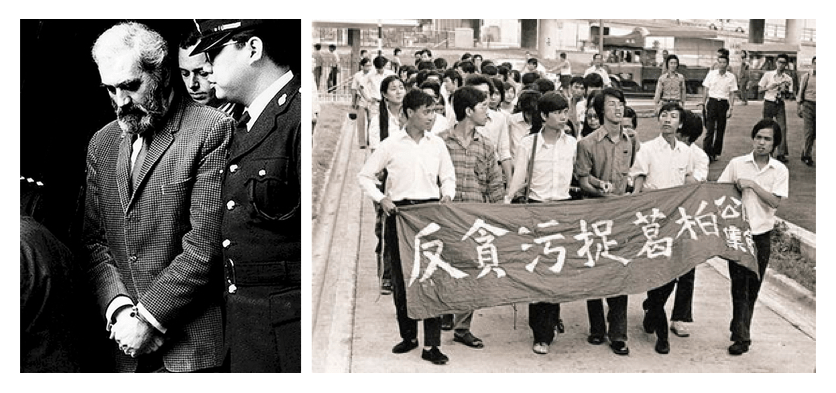
\includegraphics[width=0.7\textwidth]{c04/h-klesson1-004.png}
    \caption{七十年代「反貪污、捉葛柏」運動(圖片來源:維基百科)} 
\end{figure}

這些年輕人有的走進基層,搞起新一代的社會運動,例如協助低下階層爭取權益,要求把中文列為法定語言,還有反貪污的抗議運動。對這些在香港成長的新一代來說,香港從來都是他們的家,他們對社會改革的呼聲理直氣壯。即使沒有涉足政治的大多數年輕人,也受惠於香港經濟的急速擴張,中產階級慢慢形成。香港首個大型私人屋苑美孚新邨,也在七十年代落成。相信通過自身努力和把握機會,便可以向上流動改善生活環境,成為許多人願意相信的社會共識,也把香港和正處於計劃經濟和文化大革命的中國大陸區分開。身為香港人,成為一件值得自豪的事情。有別於中國大陸的香港認同,由此而起。

\rule[-10pt]{15cm}{0.05em}

伸延閱讀:

呂大樂(2012):《那似曾相識的七十年代》,香港:中華書局。

谷淑美(2009):〈從移民政策的歷史軌跡看香港身分認同的構成 (1950-80)〉,馬家輝等編《本土論述 2009:香港的市民抗爭與殖民地秩序 》,漫遊者文化事業股份有限公司。

周永新(2019):《香港人的身份認同和價值觀》,香港:中華書局(香港)有限公司。

Lau, Siu-Kai (1982), \textit{Society and Politics in Hong Kong}. Hong Kong: The Chinese University Press.